\documentclass{article}
\usepackage[utf8]{inputenc}
\usepackage[dvips]{graphicx}
\usepackage{a4wide}
\usepackage{amsmath}
\usepackage{euscript}
\usepackage{amssymb}
\usepackage{amsthm}
\usepackage{amsopn}
\usepackage{mathtools}

\theoremstyle{definition}
\newtheorem*{definition}{Definition}
\newtheorem{theorem}{Theorem}
\newcommand{\cis}{\mbox{cis}}
\newcommand{\vv}{\ensuremath{\vec{v}}}
\newcommand{\vu}{\ensuremath{\vec{u}}}
\newcommand{\vw}{\ensuremath{\vec{w}}}
\newcommand{\vx}{\ensuremath{\vec{x}}}
\newcommand{\vy}{\ensuremath{\vec{y}}}
\newcommand{\vb}{\ensuremath{\vec{b}}}
\newcommand{\vo}{\ensuremath{\vec{0}}}
\newcommand{\va}{\ensuremath{\vec{a}}}
\newcommand{\ve}{\ensuremath{\vec{e}}}
\newcommand{\deriv}{\frac{d}{dz}}

\usepackage{halloweenmath, tikzsymbols}

\newcommand{\R}{\mathbb{R}}
\newcommand{\Z}{\mathbb{Z}}
\newcommand{\C}{\mathbb{C}}
\newcommand{\N}{\mathbb{N}}
\newcommand{\Q}{\mathbb{Q}}
\newcommand{\Arg}{\mbox{Arg}}
\newcommand{\Log}{\mbox{Log}}

\newcommand{\cs}[1]{\color{blue}{#1}\normalcolor}
\newcommand{\ab}[1]{\color{red}{#1}\normalcolor}

\title{Complex Analysis}
\author{ajbergquist }
\date{August 2021}

\begin{document}
\fbox{proposition} Given integers $m$ and $n$,
$$\int_0^{2\pi}e^{im\theta}e^{-in\theta}d\theta = \Big\{
\begin{array}{cc}
     & 0 \mbox{ when } m \ne n \\
     & 2\pi \mbox{ when } m = n\\
\end{array}.$$
\fbox{proof} First, suppose that $m\ne n$. By the properties of exponential functions, we can simplify the integrand: $e^{im\theta}e^{-in\theta} = e^{i\theta(m-n)}.$ Furthermore, by Euler's theorem, we can rewrite this as $e^{i\theta(m-n)} = \cos{\theta(m-n)}+i\sin{\theta(m-n)}.$ Substituting and seperating the real and imaginary parts of the integral we have 
$$ \begin{array}{cc}
     &  \int_0^{2\pi}e^{im\theta}e^{-in\theta}d\theta
     = \int_0^{2\pi}\cos{\theta(m-n)}d\theta + i\int_0^{2\pi}\sin{\theta(m-n)}d\theta \\
     & -1/(m-n)\sin(\theta(m-n))\Big|_0^{2\pi} + i/(m-n)\cos(\theta(m-n))\Big|_0^{2\pi\\}.
    \end{array}
$$
By the closure property of integers under addition, $m-n\in \Z$. Furthermore, $\sin(2\pi n) = 0$ and $\cos(2\pi n) = 1$ for all $n\in \Z$ (including $n= 0$). Hence this reduces to $\int_0^{2\pi}e^{im\theta}e^{-in\theta} = 1-1 + 0-0 = 0$. Hence the proposition holds in the case where $m \ne n$.\\

Now suppose that $m = n$. In this case, the integrated reduces to $e^{im\theta}e^{-in\theta} = e^{im\theta}e^{-im\theta}= e^{i\theta(m-m)} = e^0 = 1$. Evaluating the integral, we find $\int_0^{2\pi}1d\theta = 2\pi$. Hence the proposition holds when $m = n$ as well.\\
Q.E.D.\\

\cs{5/5}


\fbox{proposition} Let $C$ denote the right hand half of the circle $|z| = 2$ in the counterclockwise direction, and note that two parametric representations for $C$ are 
$$z = z(\theta)= 2e^{i\theta}, (-\frac{\pi}{2}\le \theta \le \frac{\pi}{2})$$
and $$z = Z(y) = \sqrt{4- y^2} + iy, (-2\le y \le 2).$$
Verify that $Z(y) = [\phi(y)]$ where $\phi(y) = \arctan{\frac{y}{\sqrt{4-y^2}}}$ and $(-\frac{pi}{2}< \arctan t < \frac{pi}{2}).$ Also, $\phi(y)$ has a positive derivative inside the parameters.\\


\fbox{proof} First, we make the substitution $\theta = \phi(y)$. So we have $z(\phi(\theta)) = 2\exp(i\arctan{\frac{y}{\sqrt{4-y^2}}}).$ By definition of the complex arctangent and the properties of the exponential and complex functions of complex variables, this is just 
$$\begin{array}{cc}
     & 2\exp\left(\left[i\frac{i}{2} = -1/2\right]\log{\frac{i+\frac{y}{\sqrt{4-y^2}}}{i-\frac{y}{\sqrt{4 - y^2}}}}\right) = 2\left(\exp\left(\log{\frac{i+\frac{y}{\sqrt{4-y^2}}}{i-\frac{y}{\sqrt{4-y^2}}}}\right) \right)^{-\frac{1}{2}}  \\
     & = 2\left(\frac{i+\frac{y}{\sqrt{4-y^2}}}{i-\frac{y}{\sqrt{4-y^2}}}\right)^{-\frac{1}{2}} = \pm2\sqrt{A},
\end{array} $$
where (and manipulating) $$\begin{array}{cc}
     & A =\frac{i-\frac{y}{\sqrt{4-y^2}}}{i+\frac{y}{\sqrt{4-y^2}}} = \frac{\frac{i\sqrt{4-y^2}-y}{\sqrt{4-y^2}}}{\frac{i\sqrt{4-y^2}+y}{\sqrt{4-y^2}}} \\
     & = \frac{i\sqrt{4-y^2}-y}{i\sqrt{4-y^2}+y} = \frac{i\sqrt{4-y^2}-y}{i\sqrt{4-y^2}+y}\cdot\frac{[-i\sqrt{4-y^2} + i = -(i\sqrt{4-y^2} - y)]}{-i\sqrt{4-y^2} + y} = \frac{-(i\sqrt{4-y^2} - y)^2}{4}.
\end{array}  $$
Then, since we have multiple values, we want to chose one of them (not sure if I can just do this). Choose $z(\phi(y)) = -2\sqrt{A}$. Then  $z(\phi(y)) = -2\sqrt{A} = -2\sqrt{\frac{-(i\sqrt{4-y^2} - y)^2}{4}} =  -i(i\sqrt{4-y^2}- y) = \sqrt{4-y^2}+yi = Z(y).$\\
Q.E.D.\\

\fbox{alternative proof} The algebra in that one was awful, but I already had it typed there and didn't want to get rid of it. This is a geometric proof.\\
Let $\theta = \phi(y) = \arctan{\frac{y}{\sqrt{4-y^2}}}$. Using the definition of arctangent as the angle which produces the ratio between the sin and cosine of an angle, that is, opposite and adjacent of a right triangle, we can find the sin and cosine of the angles, we have:
\begin{figure}[htbp]
\centerline{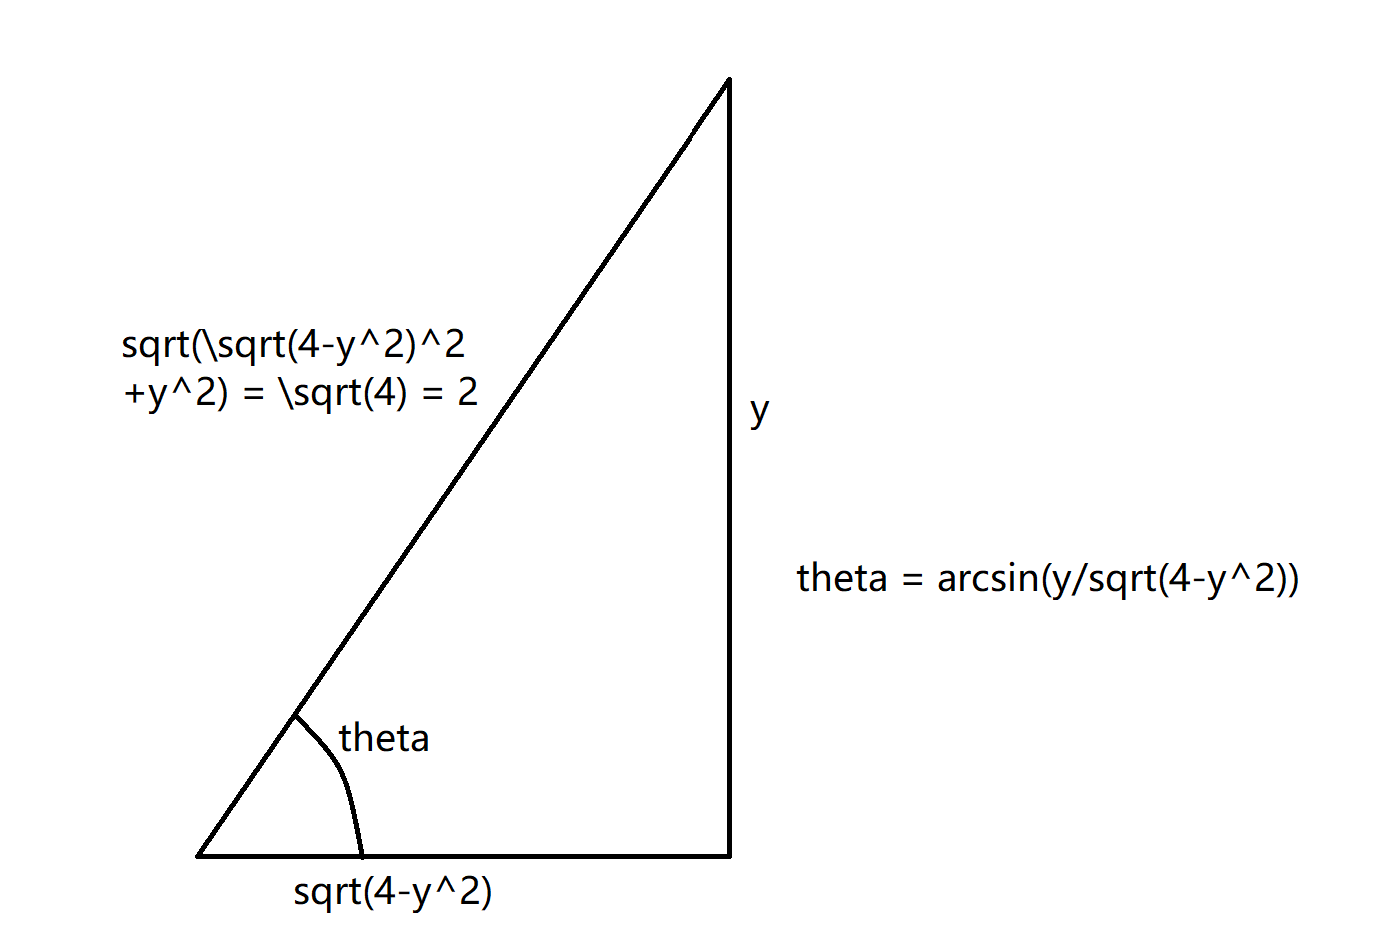
\includegraphics[scale=0.5]{triangle.png}}
\caption{right triangle}
\label{fig}
\end{figure}\\
Recall from trigonometry that $\sin\theta$ is the opposite divided by the hypotenuse. So we have $\sin\theta = y/2$. Furthermore, since $\cos\theta$ is the adjacent over the hypotenuse, we have $\cos\theta = \sqrt{4-y^2}/2$. Using the $\theta$ given by the arctangent and substituting it into $z(\theta)$, we have $z(\phi(y) = \theta) = 2e^{i\theta}$. Then by Euler's formula and what we have reasoned geometrically, $z(\phi(y)) = 2(\cos\theta + i\sin\theta) = 2(\sqrt{4-y^2}/2 + iy/2) = \sqrt{4-y^2} +iy = Z(y)$.
Q.E.D.\\

\cs{5/5}

\fbox{proof that $\phi'(y) > 0$}
Let $f(y) = y(4-y^2)^{\frac{-1}{2}}$ for convenience. To show that $\phi(y)$ has a positive derivative on the interval, we use the previously proven properties of arctangents and the chain rule to find that 
$$\begin{array}{cc}
     & \phi'(y) = \frac{d}{dy}\arctan{\frac{y}{\sqrt{4-y^2}}} = \frac{f'(y)}{1+f(y)^2} = \frac{(4-y^2)^{\frac{-1}{2}}(1+(4-y^2)^{\frac{-1}{2}}y)}{1+(4-y^2)^{\frac{-1}{2}}y}\\
     & = (4-y^2)^{-1/2}.
\end{array}$$
Hence $\phi'(y)$ does not exist for $y = \pm 2$. It is, however, always positive, as $(4-y^2)^{-1/2}$ is always positive.\\
Q.E.D.

\fbox{proposition} Let $y(x)$ be a real valued function defined on the interval $0\le x\le 1$ by means of the equations 
$$ y(x) = \Big\{\begin{array}{cc}
     & x^3\sin(\pi/x)\mbox{ when }0<x\le 1 \\
     & 0 \mbox{ when } x = 0\\
\end{array}.$$
\begin{itemize}
    \item[a. ] Then the equation $z = x + iy(x)\hspace{0.5cm} (0\le x \le 1)$ represents an arc $C$ that intersects the real axis at the points $z = 1/n$ for $n\in \N$, and $z = 0$.
    \item[b. ] Furthermore, $C$ is a smooth arc when $x> 0$. 
    \end{itemize}
\fbox{proof a} To show that $C$ is an arc, we must first show that its real and imaginary parts are continuous functions of the real parameter, which in this case is $u(x) = x$ and $v(x) = y(x)$. Since polynomial functions, sine functions are continuous, and since rational functions are continuous besides when the denominator is zero, it follows that $y(x)$ is continuous on the interval $(0,1]$ it remains to be shown that $y(x)$ is continuous at $x = 0$. To verify this, we need to show that the limit of $y(x)$ as $x$ approaches zero exists and is zero, and also that $y(0)$ is defined. We get the last thing by definition of $y$. To show that the limit exists and is zero, let $\epsilon > 0$, and consider $\delta = \sqrt[3]{\epsilon},$ and suppose that $|x-0|< \sqrt[3]{\epsilon}$. Then cubing both sides and using properties of absolute values, we have $|x^3|< \epsilon$. Furthermore, since $x^3 \le |x^3|$, it follows that $x^3\sin(\pi/x) \le x^3 < \epsilon$. Then by definition of a limit, $\lim_{x\rightarrow 0}y(x) = 0.$ \cs{You could also use the Squeeze Theorem here.} So the limit exists and is what it should be. Since the real and imaginary parts of $C:z(x)$ are continuous functions of $x$, it follows that $C$ is an arc.\\
Now to show that $C$ intersects the real axis at $z = 0,1/n$ for natural numbers $n$. Suppose $z = 0$. Then by definition of $z$, $0 = x + y(x)i$. Then by definition of equality for complex numbers $x = 0$. Furthermore, by construction $y(0)=0$, so this is consistent, and the imaginary part of $z$ is zero, hence $z$ is real and $C$ crosses the real axis at $z = 0$.\\
Suppose that $z = 1/n = x + y(x)$. Then by definition of function equality, since $1/n\in \R$, $x = 1/n$. Furthermore, since $1/n\in (0,1]$ for all $n\in \N$, $y(1/n) = x^3[\sin(\pi/(1/n))= \sin(n\pi)].$ Since $\sin(n\pi) = 0$ for all $n
\in \N$ (this can be seen geometrically on the unit circle), it follows that $\sin(n\pi) = 0$ and hence $y(1/n) = x^3(0) = 0$. Then since $y(1/n) =0$ is the imaginary part of $z$ when $z = 1/n$, it follows that $C$ crosses the real axis at $z = 1/n$.\\
Q.E.D. \cs{Are those the *only* places $z$ is 0?}

\fbox{proof b} To show that $C$ is smooth, we need to show that $z'(t)$ is continuous for all $t\in[0,1]$, and nonzero for all $t\in (0,1)$. Since $x\ne 0$, we only care about $y(x)$ when $y(x) = x^3\sin(\pi/x)$. So we have $z = [u(x) = x] + i[v(x) = x^3\sin(\pi/x)]$ Using rules of complex differentiation, we have $z'(x) = u'(x) + iv'(x) = 1 + v'(x)$. By definition of equality in the complex numbers $z'(x)$ cannot be zero, as the real part is constant at $1$. It remains to be shown that $z'(t)$ is continuous, that is, that $u'(x) = x$ and $v'(x) = y'(x)$ is continuous. Taking the derivative of $y'(x)$ for $x\in (0,1]$, we have $y'(x) = \frac{d}{dx}(x^3\sin(\pi/x)) = 3x^2\sin(\pi/x) -\pi x\cos(\pi/x),$ when $0<x\le 1$ We know from calculus that these functions are continuous on this interval, but it remains to be shown that the derivative exists at $x = 0$. The derivative of a constant is zero. \cs{That's a little misleading here. If a function is constant *on an interval*, its derivative is 0. You need to apply the definition of the derivative at $x=0.$} Hence to show that $y'(x)$ is continuous at $x = 0$, we need to show that the limit of $y'(x)$ as $x$ approaches zero is in fact zero. \\

Before proving this, there are a couple things that will probably help. First, we want to view $y'(x)$ as the sum of two functions: $y'(x) = [f(x) = x^2\sin(\pi/x)] + [g(x) = -\pi x\cos(\pi/x)]$. From calculus we know that limits can be "distributed" over addition. So in order to establish continuity at $x= 0$, in showing that $\lim_{x\rightarrow 0}y'(x) = 0$ that $\lim_{x\rightarrow 0}f(x) = 0$ and $\lim_{x\rightarrow 0}g(x) = 0$. So the proof reduces to showing that this is the case.\\

Note that since $\sin(t)$ and $\cos(t)$ are always in $[-1,1]$ for all $t\in \R$, it follows that $|3x^2\sin(\pi/x)|\le |3x^2|$ and $|-\pi x\cos(\pi/x)| <|\pi x|$ This will be helpful when proving these limits.\\

Let $\epsilon > 0$. Consider $\delta = \sqrt{\epsilon/3}$. Suppose $|x - 0| = |x| < \sqrt{\epsilon/3}$. Then it follows that $3|x|^2 = |3x^2| < \epsilon$. Using the inequality from the last paragraph it follows that $|3x^2\sin(\pi/x) - 0| < \epsilon$. Then for all $\epsilon>0$ there exists some $\delta$ such that $|x-0| <\delta$ implies $|f(x) - 0| < \epsilon$. By definition of a limit, $\lim_{x\rightarrow 0}f(x) = 0$. \cs{Or use the Squeeze Theorem.}\\

Once again, let $\epsilon > 0$. Consider $\delta = \epsilon/\pi$. Suppose $|x-0| < \epsilon/\pi$. Then $\pi|x| = |\pi x| < \epsilon$. Substituting in and using the inequalities from two paragraphs ago, $|-\pi x \cos(\pi/x)| < \epsilon$. Hence $\lim_{x\rightarrow 0}g(x) = 0$.\\

Then, as we have shown, it follows that $\lim_{x\rightarrow 0}y'(y) = 0$, hence $y'(x)$ is continuous at $x =0$.\\

Since $y'(x)$ exists and is nonzero at all $x\in [0,1]$, it follows that $C:z(x)$ for $x\in [0,1]$ is in fact a smooth curve.

Q.E.D.

\cs{Existence of $z'(0)$ is still a question here. 9.5/10}

\cs{14.5/15}

\end{document}


